\documentclass[letterpaper]{article}

\usepackage{natbib,alifeconf}  %% The order is important

\usepackage{hyperref}

\usepackage{subcaption}

\usepackage{hhline}

\ifdefined\mydraft
\mydraft
\fi

\graphicspath{{img/}}

% *****************
%  Requirements:
% *****************
%
% - All pages sized consistently at 8.5 x 11 inches (US letter size).
% - PDF length <= 8 pages for full papers, <=2 pages for extended
%    abstracts.
% - Abstract length <= 250 words.
% - No visible crop marks.
% - Images at no greater than 300 dpi, scaled at 100%.
% - Embedded open type fonts only.
% - All layers flattened.
% - No attachments.
% - All desired links active in the files.

% Note that the PDF file must not exceed 5 MB if it is to be indexed
% by Google Scholar. Additional information about Google Scholar
% can be found here:
% http://www.google.com/intl/en/scholar/inclusion.html.


% If your system does not generate letter format documents by default,
% you can use the following workflow:
% latex example
% bibtex example
% latex example ; latex example
% dvips -o example.ps -t letterSize example.dvi
% ps2pdf example.ps example.pdf


% For pdflatex users:
% The alifeconf style file loads the "graphicx" package, and
% this may lead some users of pdflatex to experience problems.
% These can be fixed by editing the alifeconf.sty file to specify:
% \usepackage[pdftex]{graphicx}
%   instead of
% \usepackage{graphicx}.
% The PDF output generated by pdflatex should match the required
% specifications and obviously the dvips and ps2pdf steps become
% unnecessary.


% Note:  Some laser printers have a serious problem printing TeX
% output. The use of ps type I fonts should avoid this problem.


\title{TODO TITLE}
\author{Matthew Andres Moreno$^{1}$ \and Charles Ofria$^{1}$ \\
\mbox{}\\
$^1$BEACON Center, Michigan State University, East Lansing, MI 48824 \\
mmore500@msu.edu} % email of corresponding author

% For several authors from the same institution use the same number to
% refer to one address.
%
% If the names do not fit well on one line use
%         Author 1, Author 2 ... \\ {\Large\bf Author n} ...\\ ...
%
% If the title and author information do not fit in the area
% allocated, place \setlength\titlebox{<new height>} after the
% \documentclass line where <new height> is 2.25in



\begin{document}
\maketitle

\begin{abstract}

Genetic programming and artificial life systems commonly employ tag-matching schemes to determine interactions between model components.
%Criteria to determine affinity between tags %TODO
However, the implications of criteria used to determine affinity between tags with respect to constraints on emergent connectivity, canalization of changes to connectivity under mutation, and evolutionary dynamics have not been considered.
We highlight differences between tag-matching criteria with respect to geometric constraint and variation generated under mutation. 
We find that tag-matching criteria can influence the rate of adaptive evolution and the quality of evolved solutions.
Better understanding of the geometric, variational, and evolutionary properties of tag-matching criteria will facilitate more effective incorporation of tag matching into genetic programming and artificial life systems.
By showing that tag-matching criteria influence connectivity patterns and evolutionary dynamics, our findings also raise fundamental questions about the properties of tag-matching systems in nature.

\keywords{Genetic Programming \and Event-driven Genetic Programming \and Tag-based Referencing \and Module-based Genetic Programming \and Artificial Gene Regulatory Networks}
% \PACS{PACS code1 \and PACS code2 \and more}
% \subclass{MSC code1 \and MSC code2 \and more}

\end{abstract}


\section{Introduction}

TODO \citep{taylor2016open}

\subsection{What is a tag?}

At a broad level, tags are labels that can be used to refer to labelees (the
tagged thing).

\subsubsection{Examples of tags}

\begin{itemize}
  \item Human culture (probably don't want to draw too many examples from this category)
    \begin{itemize}
      \item We name our offspring, which is useful for later referring to them.
            Names are often repeated across individuals (e.g., we'll be seeing an
            uptick in `Arya's post-GoT). Context + multi-level naming (first, middle,
            last in 20th century American culture) is important for resolving collisions.
    \end{itemize}
  \item Software development
    \begin{itemize}
      \item In software development, we label and refer to lots of things! In this
            domain, tags are precise: after labeling (tagging) something, subsequent
            referrals to those labeled things must be \textit{exact}. Inexactness
            in a reference typically results in syntactic errors.
      \item Common uses: labeling and specifying locations in memory, custom data
            structures (e.g., structs, classes, etc), functions, libraries/modules,
            language constants/built-ins, program entry points, locations in an
            instruction sequence (e.g., function names, looping, conditionals etc).
    \end{itemize}
  \item Chemistry?
  \item Biology?
    \begin{itemize}
      \item cell signaling
      \item protein folding
    \end{itemize}
\end{itemize}

\subsubsection{What are the benefits of tags/tag-based referencing?}

\begin{itemize}
  \item Hypothesis: Inexactness allowed by tag-based referencing makes these references
        more robust to minor genetic perturbations, smoothing the genotype-phenotype
        mapping relative to more traditional memory-indexing techniques (pulled from
        2019 Tag-access memory abstract).
  \item We don't need to know/lock-in the architecture of what our tags are referencing.
        If a referent (e.g., module) is deleted, it doesn't invalidate any of the
        in-program references (e.g., module calls). The same is true for creating
        a new referent. For example, using tags to reference program modules allows
        you to mutate the number of modules in the program without (necessarily)
        breaking existing references.
  \item Hypothesis: Tag-based referencing should help to enable the duplication/
        deletion of referents (e.g., modules), which should improve capacity for
        complexity to evolve (i.e., duplication is often cited as important in the
        evolution of complex features).
\end{itemize}


\section{Methods}

Each tag was represented as an ordered, fixed-length bitstring,
\begin{align*}
t = \langle t_0, t_1, t_2, \dots, t_{n-2}, t_{n-1} \rangle
\end{align*}
where
\begin{align*}
\forall i, t_i \in \{0, 1\}.
\end{align*}
In all experiments, we used 32 bit tags.

For consistency between metrics, we bound all metrics between 0 and 1.

\subsection{Integer Metric}

This metric is inspired by \citep{spector2011tag}.
They used positive integers between 0 and 100 to name referents.
Queries were provided the referent that had the next-larger value, wrapping around from 100 back to 0.

In this metric, we compare tags according to their value as an unsigned integer according to the following representation $f$,
\begin{align*}
f(t)
= \sum_{i=0}^{n-1} t_i \times 2^i.
\end{align*}

The distance metric $I$ between two length-$n$ tags $t$ and $u$ is
\begin{align*}
I(t, u) =
\begin{cases}
  \frac{2^n - f(t) + f(u)}{2^n}, & \text{if } f(t) > f(u), \\
  \frac{f(t) - f(u)}{2^n},         & \text{else} f(t) \leq f(u).
\end{cases}
\end{align*}

Note that this metric is non-commutative, i.e., it is not necessarily true that $I(t, u) = I(u, t)$.

Note also that this metric is one-dimensional.

A algorithmic advantage of this metric is that it allows for log-time matching.

\subsection{Hamming Metric}

This metric is based on the work of \citep{lalejini2019else}, originally after TODO hamming cite(?).

In this metric, we compare tags according to their bitwise hamming distance.
Mathematically speaking for tags $t$ and $u$ we compute the distance according to the metric $M$ as,
\begin{align*}
M(t, u)
= \frac{
  \#\{ i : t_i \neq u_i, i=0, \dots ,n-1\}
}{
  n
}
\end{align*}

This metric is commutative and $n$-dimensional.

\subsection{Hash Metric}

This metric is original to the our paper and meant to serve as a control.

The an arbitrary, but determinsitic value, uniformly distributed between 0 and 1.

We rely on the \texttt{hash\_combine} function, adapted from BOOST (TODO cite).

for two values \texttt{v1} and \texttt{v2}, \texttt{hash\_combine} is defined as follows
\begin{verbatim}
unsigned int hash_combine(
  unsigned int v1,
  unsigned int v2
) {
  return v1 ^ (
    v2 * 0x9e3779b9
    + (v1 << 6) + (v1 >> 2)
  );
}
\end{verbatim}

We compute the hash value of a tag as follows
\begin{verbatim}
unsigned int h(unsigned char *tag) {
  unsigned int result = tag[0];
  for (int i = 1; i < 4; ++i){
    result = hash_combine(result, t[i]);
  }
  return result;
}
\end{verbatim}
where \texttt{tag} is the tag's bitstring stored as an array of bytes.

To compute the metric $H$ we then call \texttt{hash\_combine} to combine the hash values of the tags $t$ and $u$
\begin{align*}
H(t, u) = \texttt{hash\_combine( h(}t\texttt{), h(}u\texttt{))}
\end{align*}

Note that this is not commutative.

\subsection{Streak Metric}

This metric was originally proposed by \citep{downing2015intelligence}.
Downing claims that it exhibits
It is computed according to the ratio between the longest contiguously matching substring among two bitsets and the longest contiguously mismatching substring among those two bitsets.
Downing claims that this metric exhibits greater robustness compared to integer and hamming distance metrics using mutational walk experiments but does not demonstrate it in an evolving system.

We define the greatest contiguously-matching length of $n$-long bitstrings $t$ and $u$ as follows,
\begin{align*}
m(t, u) = \max(\{i - j \forall i, j \in 0..n-1 \mid \forall q \in i..j, t_q = u_q \})
\end{align*}

We define the greatest contiguously-mismatching length as follows,
\begin{align*}
n(t, u) = \max(\{i - j \forall i, j \in 0..n-1 \mid \forall q \in i..j, t_q \neq u_q \})
\end{align*}

The streak metric $S'$  with tags $t$ and $u$
\begin{align*}
S'(t, u)
= \frac{ p(n(t,u)) }{p(m(t,u)) + p(n(t,u))}.
\end{align*}
where $p$ approximates the probability of a contiguously-matching substring between

It is worth noting that the formula for computing the probability of a $k$-bit match or mismatch, given by Downing as follows, is actually mathematically flawed.
\begin{align*}
p_k
= \frac{n - k + 1}{2^k}
\end{align*}

The probability of a $0$-bit match according to this formula would be computed as $p_0 = \frac{n - 0 + 1}{2^0} = n + 1$ which is clearly impossible because $p_0 > 1 \forall n > 0$.
The actual can probability be achieved using a lookup table computed using dynamic programming.

However, the formula Downing presented provides a useful approximation to the probability of a $k$ bit match.
For computational efficiency and consistency with the existing literature we use clamp edge cases between 0 and 1 to yield the corrected streak metric $S$.

\begin{align*}
S(t, u) =
\max( \min( S'(t, u), 1), 0)
\end{align*}

\subsection{Uniformification}

In experiments where actual match distance values, instead of the relative ranking of match distances, were mechanistically important or reported as data we transformed each match distance function such that the distribution of match distances of randomly generated bitstring pairs would approximate the uniform distribution between 0 and 1.
We sampled 10,000 randomly generated bitstring pairs to generate a set of match distances for each metric.
To generate a corrected distance for a raw distance $r$, we simply calculated its percentile ranking in the match distance database divided by one hundred.
If the exact raw distance $r$ wasn't present in the set of sampled match distances, we applied linear interpolation.
Specifically,
\begin{align*}
 p(m_b)/100.0 + r \times \frac{m_a - r}{m_a - m_b}
\end{align*}
where $p()$ is the percentile function, $m_a$ is the next-greater match distance, and $m_b$ is the next-lower match distance.

\begin{figure}
\begin{center}

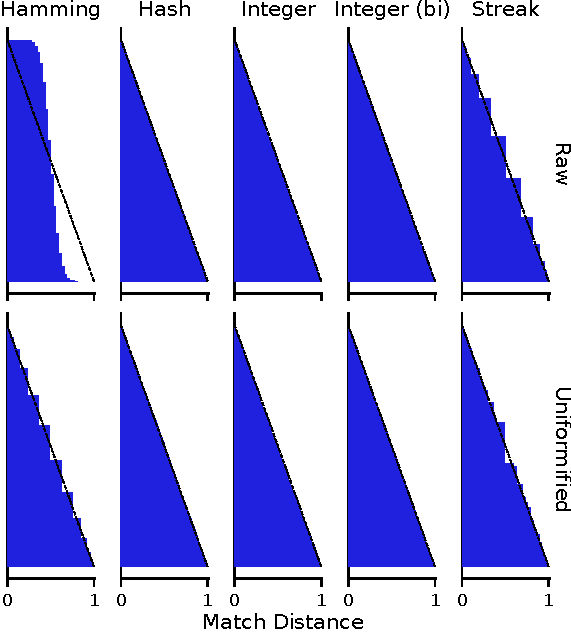
\includegraphics[width=\columnwidth]{img/uniformification/bitweight=0dot5+seed=1+title=low-score-distribution+_data_hathash_hash=75684cf1e73fb7f1+_script_fullcat_hash=d4b3b5e14a0d1350+ext=}
\caption{
Distance distributions of metrics before and after uniformification.
Dashed line indicates an ideal uniform distribution.
}
\label{fig:uniformification}

\end{center}
\end{figure}

Figure \ref{fig:uniformification} depicts the distributions of match distances between randomly sampled bitstring pairs for each metric before and after uniformification.

there's a lot of arbitrary metrics that could be created as follows
note that, for example,
\begin{align*}
f\Big( (0 \cup 1)^{32} \times (0 \cup 1)^{32} \Big) \rightarrow [0, 1]
\end{align*}

\begin{align*}
f^2\Big( (0 \cup 1)^{32} \times (0 \cup 1)^{32} \Big) \rightarrow [0, 1]
\end{align*}

What we're really interested is the ranking order of similarities over the $(0 \cup 1)^{32} \times (0 \cup 1)^{32}$ that the metric imposes, so applying a unifying transform onto the raw match distances helps to isolate that.
Plus, it provides an intuitive interpretation to match distances: a 0.01 distance match matches better than 99\% of all matches.

\subsection{Implementation}

We implemented our experimental system using the Empirical library for scientific software development in C++, available at \url{https://github.com/devosoft/Empirical}.
The code used to perform and analyze our experiments, our figures, data from our experiments, and a live in-browser demo of our system is available via the Open Science Framework at \url{https://osf.io/TODO/}.


\section{Results and Discussion}
% @AML: I would hesitate to call the Integer metric the Spector Integer metric. The underlying representation
%       is not the same, resulting in different mutational properties.

\subsection{Geometric Properties}

To gain intuition for how they might affect patterns of tag connectivity, we began by surveying geometric properties of the tag matching metrics.

\begin{figure}
\begin{center}

\begin{subfigure}[b]{0.5\linewidth}
\centering
\includegraphics[width=\linewidth]{dimensionality-statistic}
\caption{
Dimensionality statistic
}
\label{fig:dimensionality_statistic}
\end{subfigure}%
\begin{subfigure}[b]{0.5\linewidth}
\centering
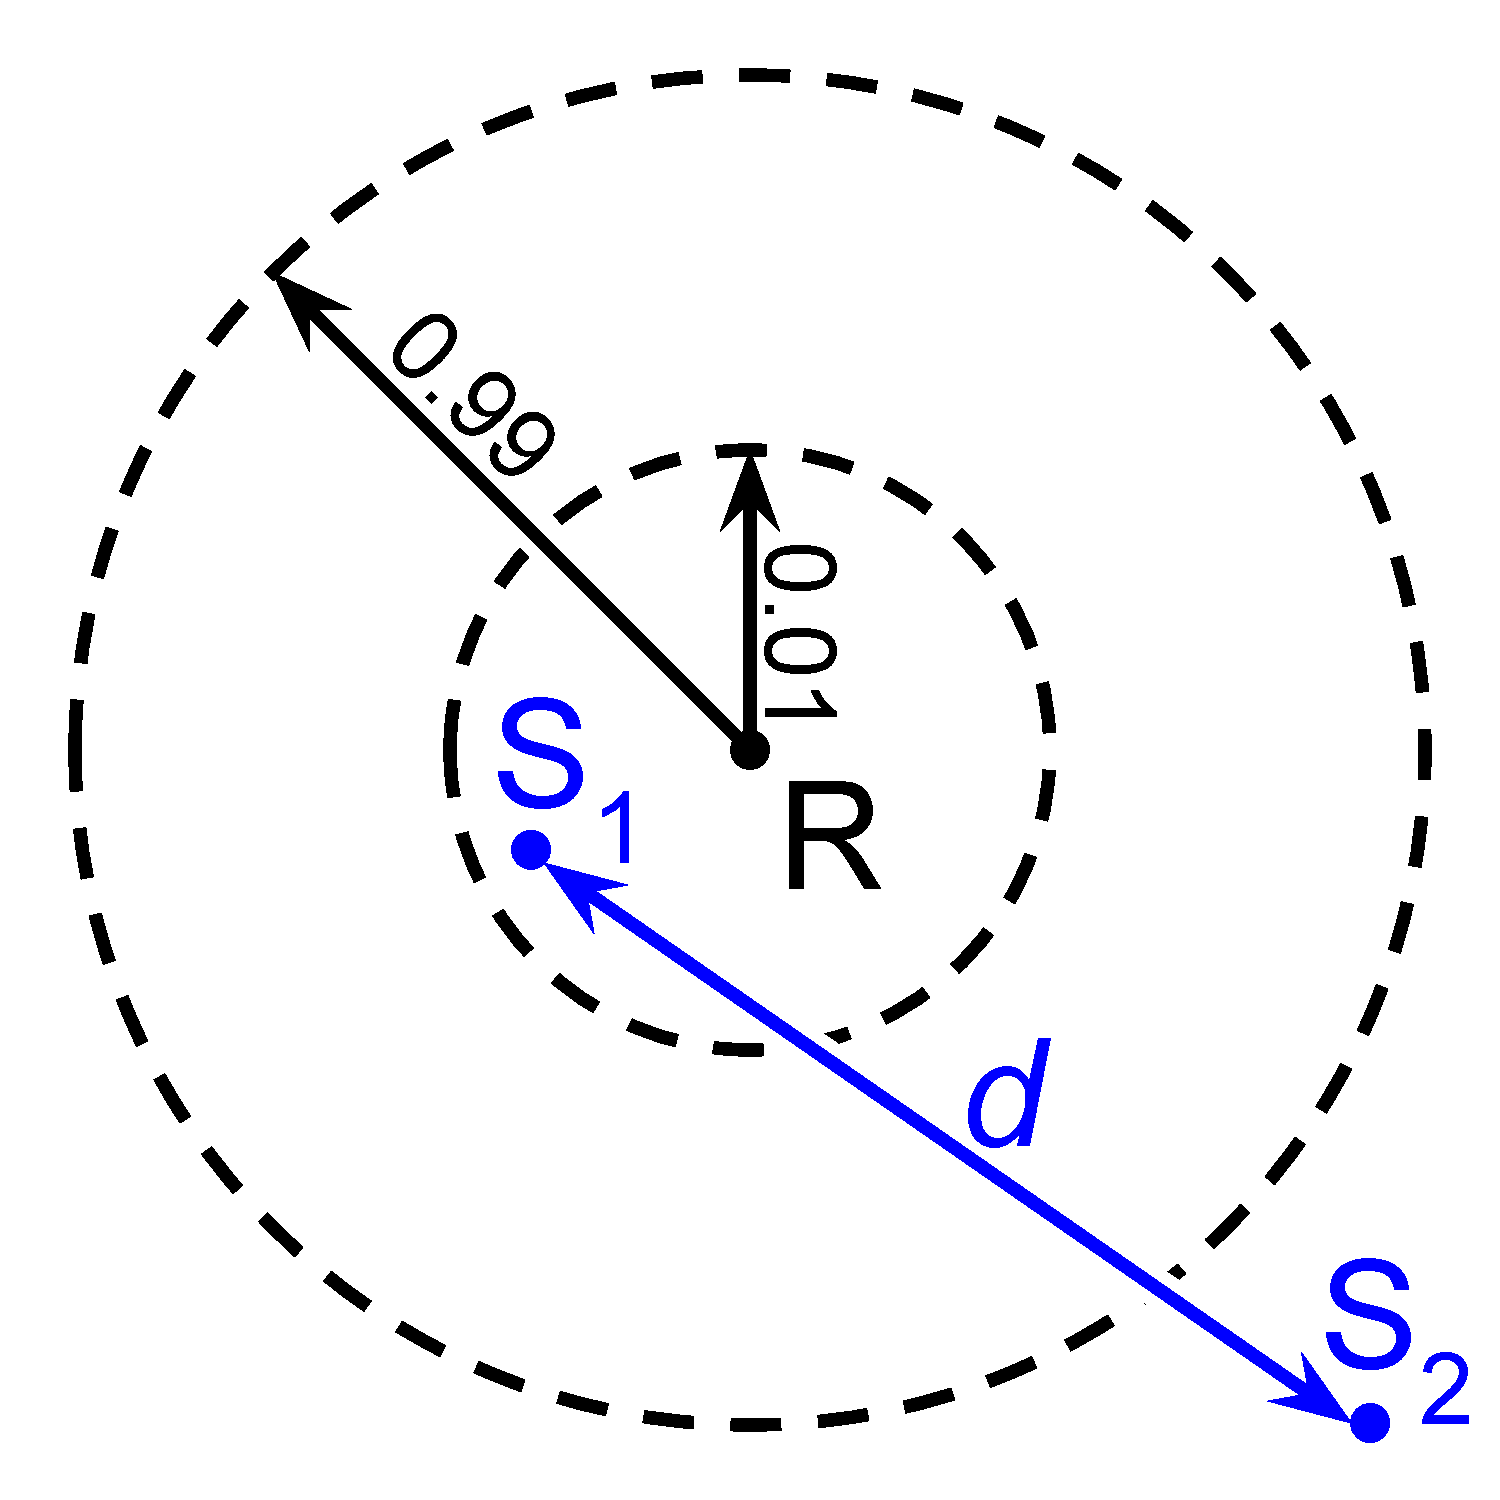
\includegraphics[width=\linewidth]{elasticity-statistic}
\caption{
Elsaticity statistic
}
\label{fig:elasticity_statistic}
\end{subfigure}

\caption{
A schematic depicting (A) the process used to generate the dimensionality statistic for each metric and (B) the process used to generate the elasticity statistic for each metric.
}
\label{fig:dimensionality_measure}

\end{center}
\end{figure}


\begin{figure*}
\begin{center}

\begin{minipage}{\linewidth}
\begin{subfigure}[b]{\linewidth}
\begin{minipage}{0.5\textwidth}
\begin{center}
\includegraphics[width=0.5\linewidth,trim=5cm 5cm 5cm 5cm, clip]{img/dimensionality-statistic}
\end{center}
\end{minipage}%
\begin{minipage}{0.5\textwidth}
\caption{
Sampling process used to measure similarity constraint.
First, a constraining tag $R$ was randomly sampled.
Then, tags were randomly drawn until two tags $S_1$ and $S_2$ with distance to $R$ less than 0.01 were obtained.
Finally, similarity constraint was measured as the distance $d$ between $S_1$ and $S_2$.
}
\label{fig:dimensionality_measure}
\end{minipage}
\end{subfigure}
\end{minipage}
\begin{subfigure}[b]{\linewidth}
\begin{minipage}{0.6\linewidth}
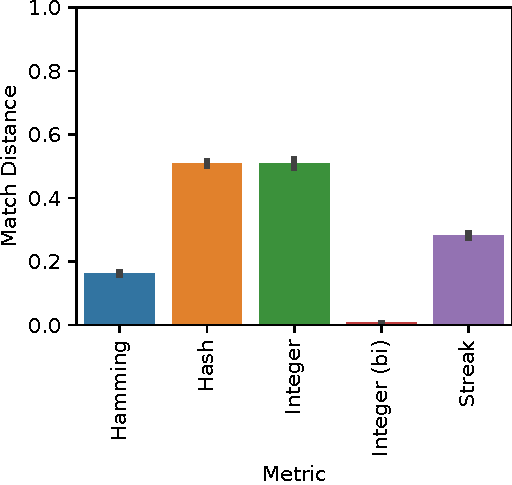
\includegraphics[width=\linewidth]{img/sphere/bitweight=0dot5+seed=1+title=dimensionality_barplot+_data_hathash_hash=c0f6c5cf854ff253+_script_fullcat_hash=03ce1e318a24a109+ext=}
\end{minipage}
\begin{minipage}{0.35\linewidth}
\caption{
Mean similarity constraint.
Error bars represent 95\% confidence intervals.
}
\label{fig:sphere_barplot}
\end{minipage}
\end{subfigure}
\begin{minipage}{\linewidth}
\begin{subfigure}[b]{\linewidth}
\centering
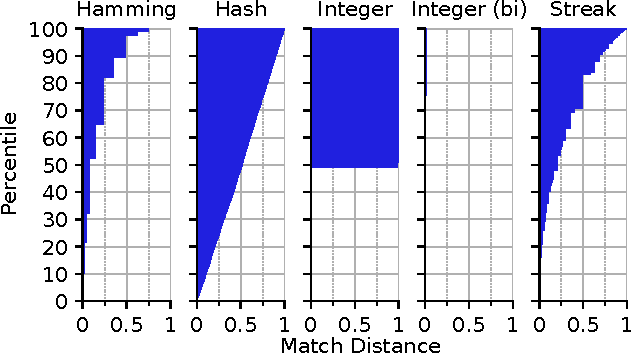
\includegraphics[width=\linewidth]{img/sphere/bitweight=0dot5+seed=1+title=dimensionality_distnplot+_data_hathash_hash=c0f6c5cf854ff253+_script_fullcat_hash=bea2a31376bf6bd0+ext=}
\begin{minipage}{0.8\textwidth}
\caption{
Distributions of sampled similarity constraint values.
Each visualization arranges individually sampled observations (thin horizontal bars) vertically in descending order.
The $y$ axis can be interpreted as ranging form the \nth{0} percentile of outcomes (bottom) to \nth{100} percentile (top) with horizontal bar width showing similarity constraint at a certain percentile.
}
\label{fig:sphere_distnplot}
\end{minipage}
\end{subfigure}
\end{minipage}

\caption{
Similarity constraint of tag-matching metrics.
Figure \ref{fig:dimensionality_measure} summarizes the sampling process used to measure similarity constraint.
Figures \ref{fig:sphere_barplot} and \ref{fig:sphere_distnplot} compare distributions of similarity constraint across metrics.
}
\label{fig:sphere}

\end{center}
\end{figure*}


To gain a sense of the dimensionality (in a loose sense) of the different tag-matching metrics, we sampled the distribution of distances between within a 0.01 match distance radius of an arbitrary target.
We used 5000 samples.
Figure \ref{fig:dimensionality_measure}a provides a cartoon summary of this process.

In a euclidean space, this would correspond to the average distance between points uniformly sampled from inside a ball (in two dimensions, a circle, and in three dimensions, a sphere).
This statistic asymptotically increases with dimensionality (TODO show this with mathematica, also try to calculate asymptote).
In one dimension, this value approximates to 0.00666667 \citep{dunbar1997average}.
In two dimensions, 0.00905415 \citep{dunbar1997average}.
In 32 dimensions, 0.0136618 \citep{dunbar1997average}.

We calculated this statistic as  0.0067569292903519994 for the bidirectional integer metric, in line with expectations.
As you can see in Figure \ref{fig:sphere_distnplot}, the distances are all bounded by the diameter of 0.02.

However, other metrics had much higher values.
For the Spector Integer metric, we approximated this value as 0.5091638296249492.
This is an artifact of the asymmetry where if you have two very similar numbers, half will be in ascending order resulting in a match distance close to 0 and half will be in descending order, resulting in a wraparound search and a match distance close to 1.
You can very clearly see these two outcomes in \ref{fig:sphere_distnplot}.
Averaging this out yields 0.5.

The uniformified hamming had a mean distance of 0.16273783884700002.
In our sample, we observed distances as high as 0.749875.
To check our intuition, we calculated this statistic for the raw hamming metric.
For numerical reasons, we raised the radius of our sampling sphere to 0.25 (e.g., with a radius of 0.01, the only result between is a perfect match and with lower radii the hits become so rare as they become difficult to sample efficiently)
in 32 dimensional euclidean space, we expect the mean distance between sampled points to be 0.341545.
In the non-uniformified hamming metric we calculate this statistic as 0.33120625.
The distortion of the uniformification is clearly affecting this statistic with respect to the hamming metric.

We calculated an even higher value of 0.2813480713989872 for the ball sampling statistic with the streak metric.
We calculated distances as high as 0.999346.

For the hash metric, we calculated the ball sampling statistic as 0.5082513209562.
A well-behaved hash should, given any set of operands, yield hash results uniformly distributed over the range.
This case holds here.
We calculated distances as high as 0.999499.

\begin{figure}
\begin{center}

\begin{subfigure}[b]{\columnwidth}
\centering
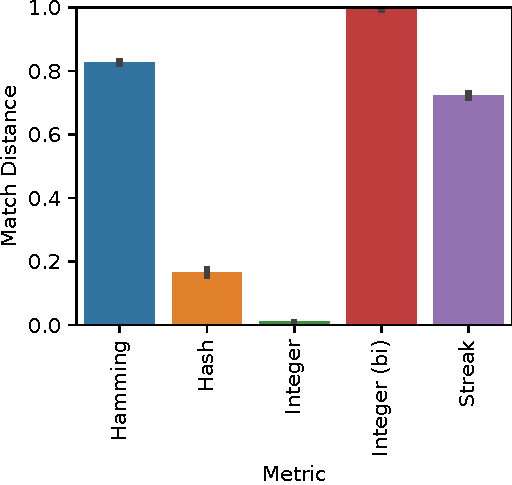
\includegraphics[width=\columnwidth]{{{sphere_reverse/bitweight=0.5+seed=1+title=dimensionality_barplot+_data_hathash_hash=7eaa832497d2f3cb+_script_fullcat_hash=03ce1e318a24a109+ext=}}}
\caption{
TODO
}
\label{fig:sphere_reverse_distnplot}
\end{subfigure}


\begin{subfigure}[b]{\columnwidth}
\centering
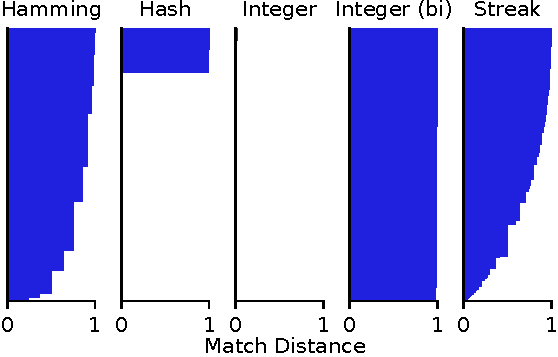
\includegraphics[width=\columnwidth]{{{sphere_reverse/bitweight=0.5+seed=1+title=dimensionality_distnplot+_data_hathash_hash=7eaa832497d2f3cb+_script_fullcat_hash=03ce1e318a24a109+ext=}}}
\caption{
TODO
}
\label{fig:sphere_reverse_barplot}
\end{subfigure}

\caption{
TODO
}
\label{fig:sphere_reverse}

\end{center}
\end{figure}


We tested the elasticity of the tag-matching metrics using a similar measure.
To gain a sense of the dimensionality (in a loose sense) of the different tag-matching metrics, we sampled the distribution of distances between a tag sampled from within a 0.01 match distance radius of an arbitrary target and a tag sampled from outside a 0.99 match distance radius of the arbitrary target.
We used 5000 samples.
Figure \ref{fig:dimensionality_measure}b provides a cartoon summary of this process.

We found that the bidirectional integer metric was highly inelastic: the smallest distance between the sampled tags was 0.980201.
The mean distance between sampled tags was 0.9932740098.
The Spector integer metric exhibited similarly uniform outcomes, except the distribution was strongly pegged to 0 because of the metric's asymmetry.
The mean statistic was 0.00998706165234.

The hamming metric exhibited greater elasticity: we observed distances between the sampled tags as low as 0.235526.
The mean distance between sampled tags was 0.8248383674.

The streak metric exhibited the greatest elasticity: we observed distances between the sampled tags as low as 0.00019998.
With this metric, a tag can have a strong attractive interaction with a second tag that a third tag it interacts attractively strongly with has a strong repulsive attraction with.
The mean distance between sampled tags was 0.7126656857120001.

The hash metric exhibited the same well-behaved uniform distribution as before, with a mean distance of 0.5102822773801999.

\begin{figure}
\begin{center}

\begin{minipage}{\linewidth}
\begin{subfigure}[b]{\linewidth}
\begin{minipage}{0.5\textwidth}
\begin{center}
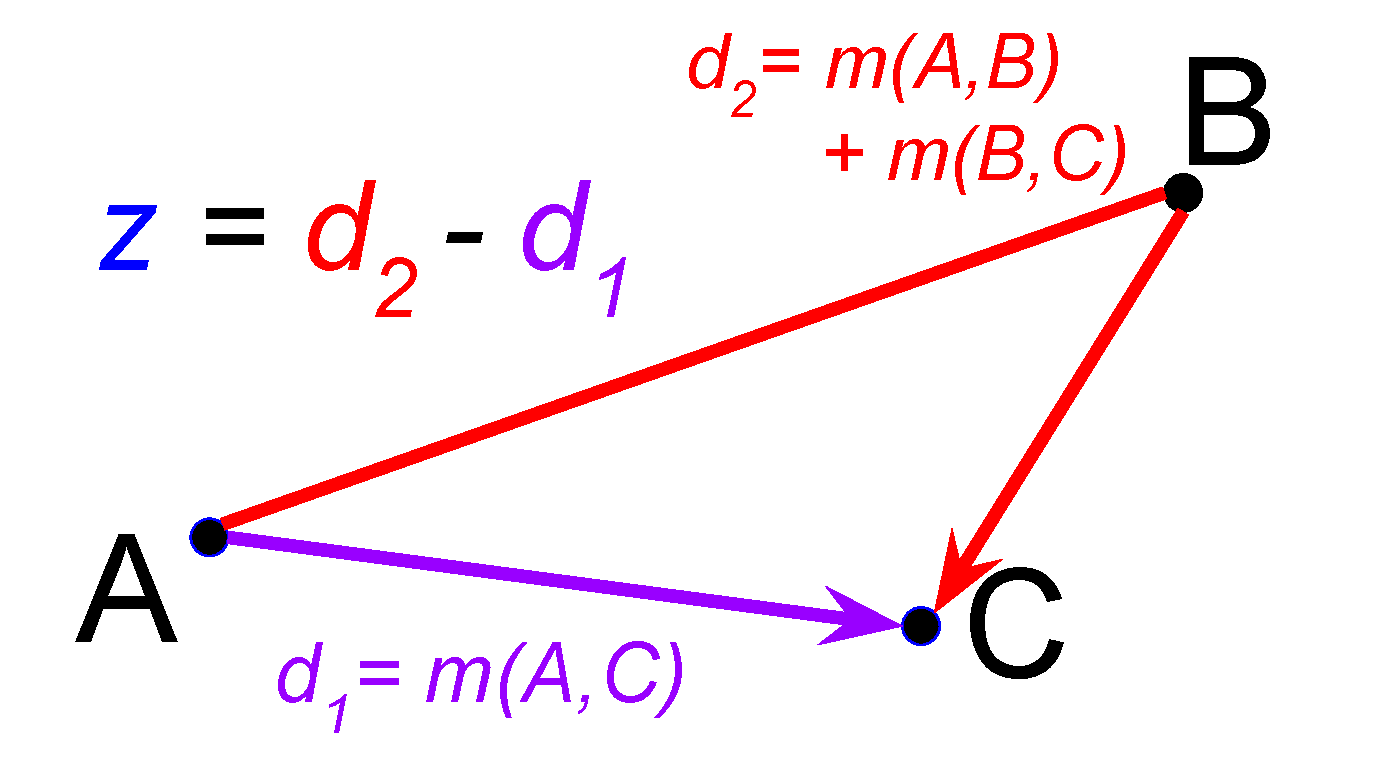
\includegraphics[width=\linewidth,trim=2cm 5cm 2cm 5cm, clip]{detour-difference}
\end{center}
\end{minipage}%
\begin{minipage}{0.5\textwidth}
\caption{
Sampling process used to evaluate detour difference, $z$.
} \label{fig:detour_difference_cartoon}
\end{minipage}
\end{subfigure}
\end{minipage}

\begin{minipage}{\linewidth}
\begin{subfigure}[b]{\linewidth}
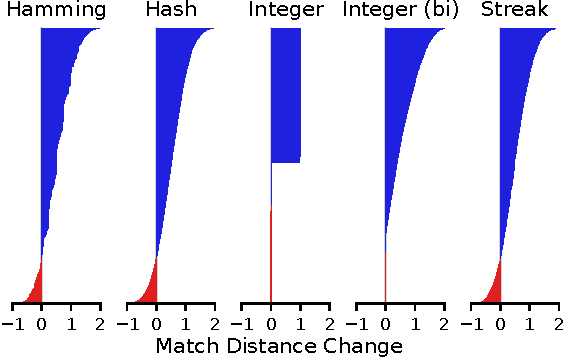
\includegraphics[width=\linewidth]{detour_difference/bitweight=0dot5+seed=1+title=low-triplet-analysis+_data_hathash_hash=6b0749ef97a58721+_script_fullcat_hash=297c4fe09078e17b+ext=}
\caption{
Distributions of detour distance difference for triplets of randomly sampled tags.
Each bar sliver represents an independently sampled observation.
A positive value (colored blue) indicates that total distance increased with the addition of an intermediate stop.
A value of exactly 0 indicates an intermediate stop had no effect on total distance.
A negative value (colored red) indicates violation of the triangle inequality: taking an intermediate stop reduced the total distance travelled.
} \label{fig:detour_difference_distribution}

\end{subfigure}
\end{minipage}

\caption{
Detour difference of tag-matching metrics.
}
\label{fig:detour_difference}

\end{center}
\end{figure}


To get a sense of the regularity, in a looses sense, of each space we uniformly sampled triplets of points $A$, $B$, and $C$.
Then, for each metric $m$ we calculated the statistic $m(A, B) + m(B, C) - m(A, C)$.
If the triangle inequality is respected this statistic should be greater than or equal to zero.
Figure \ref{fig:detour_difference} plots the distribution of this statistic for each metric.
The hamming, hash, and streak metrics show evidence of ``shortcuts'' that violate the triangle inequality.
It should be noted that the raw hamming metric does respect the triangle inequality.

\begin{figure}
\begin{center}

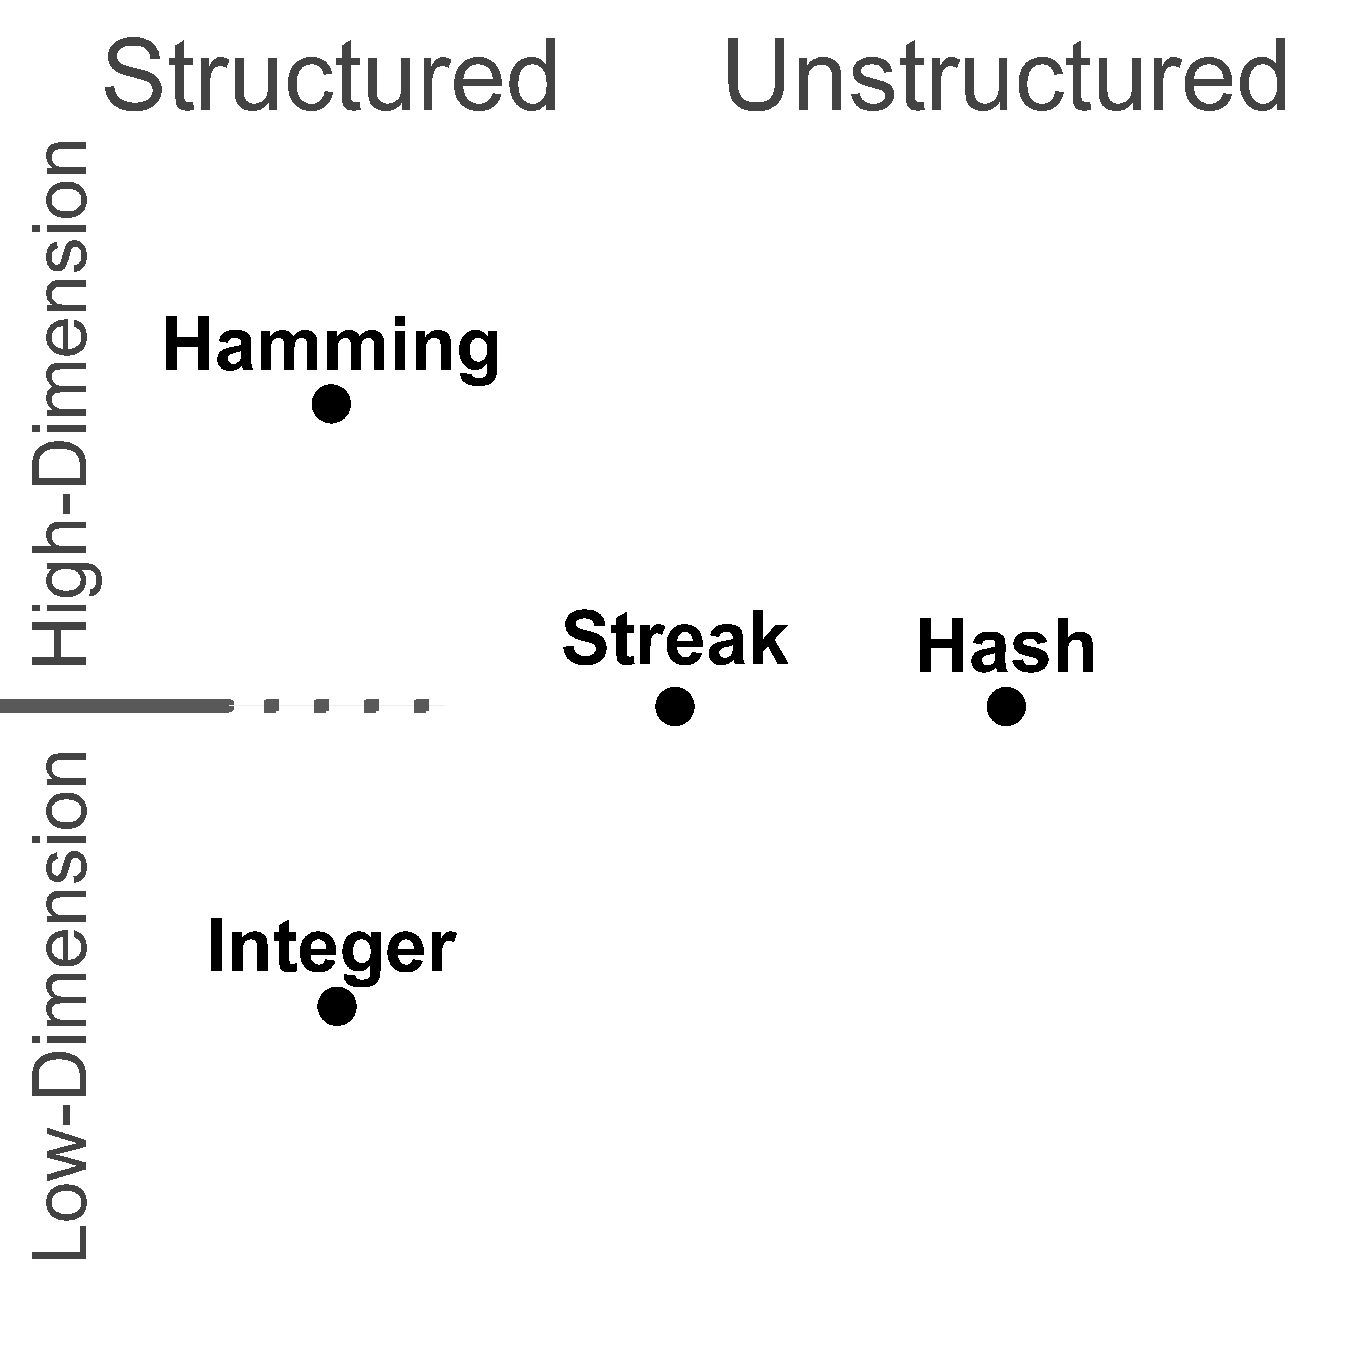
\includegraphics[width=\columnwidth]{{{img/conceptual-geometry}}}
\caption{
A conceptual schematic of the tag-matching metrics' geometric properties.
}
\label{fig:conceptual_geometry}

\end{center}
\end{figure}


\subsection{Variational Properties}

\begin{figure}
\begin{center}

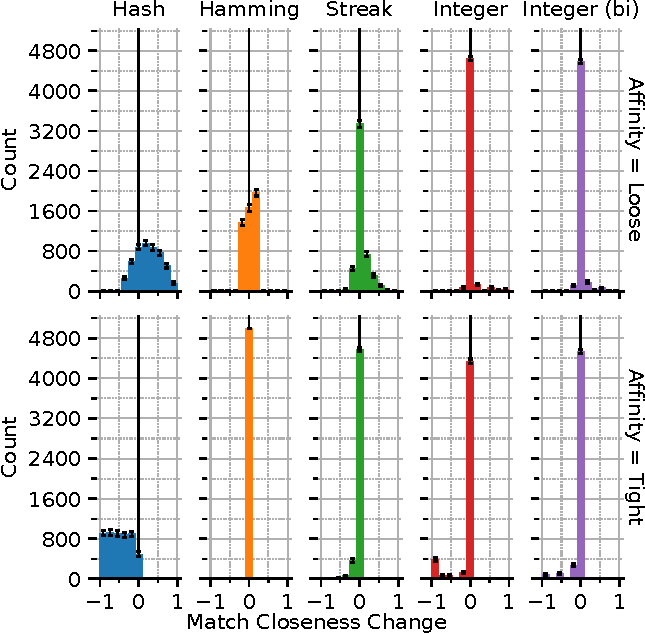
\includegraphics[width=\columnwidth]{img/mutational_step/bitweight=0dot5+seed=1+title=low-mutational-step+viz=hist+_data_hathash_hash=95a57768de56995a+_script_fullcat_hash=aa068ad24b386169+ext=}
\caption{
Distributions of mutation effects on match distance for loosely matched (pre-mutation match distance $> 0.5$) and tightly matched (pre-mutation match distance $< 0.01$) tag pairs.
Note that match closeness change (rather than mast distance change) is plotted so that better-matching mutational outcomes fall to the right and worse-matching mutational outcomes fall to the left.
Error bars are 95\% confidence intervals calculated using the Wilson score method with continuity correction \citep{newcombe1998two}.
Supplementary Figure \ref{fig:mutational_step_supp} shows the cumulative distribution of all sampled match distance changes for each metric.
}
\label{fig:mutational_step}

\end{center}
\end{figure}


We began by analyzing the distribution of single-bit mutations on match scores under the different metrics.
Figure \ref{fig:mutational_step} provides this analysis for two categories of tag pairs: loosely matched and tightly matched.
To generate the loosely matched distribution we unifomormly selected from tag pairs with a match distance > 0.5, measured their match distance, applied a one-bit mutation to the second tag, and then measured their match distance again.
To generate the tightly matched distribution we picked a target tag.
Then, we uniformly sampled a second tag with a match distance < 0.01.
We measured their match distance, applied a one-bit mutation to the second tag, and then measured their match distance again.
We sampled 5000 measurements for each affinity and each metric.

For both tight and loose affinities, although the integer metrics exhibited no perfectly neutral mutational outcomes most mutations cause very small change in the match score.
These are mutations to the least-significant bits of the bitstring.
A small fraction of mutations under these metrics, affecting the more-significant bits of the bitstring, have a stronger effect.
The integer metrics, along with the hash metric, exhibit the strongest one-step decoupling mutations under tight affinity.
The Spector integer metric, in particular, due to its asymmetrical wraparound-search inducing effect, exhibits more frequent strong decoupling mutations than the bidirectional integer metric.

The streak metric alone exhibits a portion of perfectly neutral outcomes under mutation.
The streak metric exhibits a greater fraction of mutational outcomes of non-trivial magnitude than the integer metrics with loose affinity.
Under tight affinity, the streak metric exhibits some one step strong-decoupling mutations but less intensely than the integer metrics.

The hamming metric exhibits more uniformity in the magnitudes of mutational effects than other metrics under both tight and loose affinities.
The hamming metric exhibits no perfectly neutral mutational outcomes.
(Without uniformification, all hamming metric mutations are of excactly the same magnitude with respect to match score).

The hash metric exhibits the greatest fraction of non-trivial mutational effects and exhibits some mutational intensities as extreme as the integer metrics.

\begin{figure*}
\begin{center}

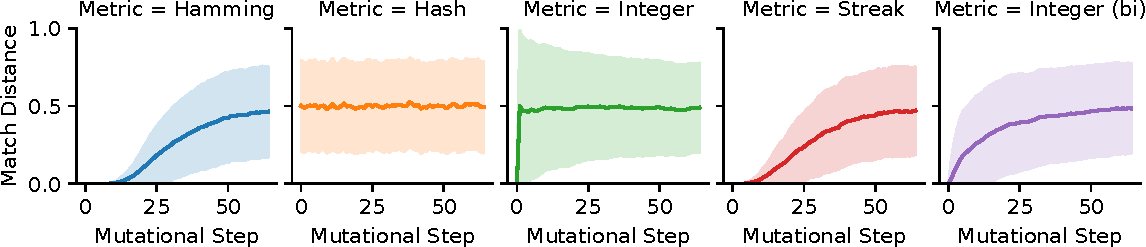
\includegraphics[width=\textwidth]{{{mutational_walk/bitweight=0.5+seed=1+title=mutational_walk_lineplot+_data_hathash_hash=ff15c8831d4f9288+_script_fullcat_hash=c872df869f05035a+ext=}}}
\caption{
TODO
}
\label{fig:mutational_walk_lineplot}

\end{center}
\end{figure*}

\begin{figure}
\begin{center}

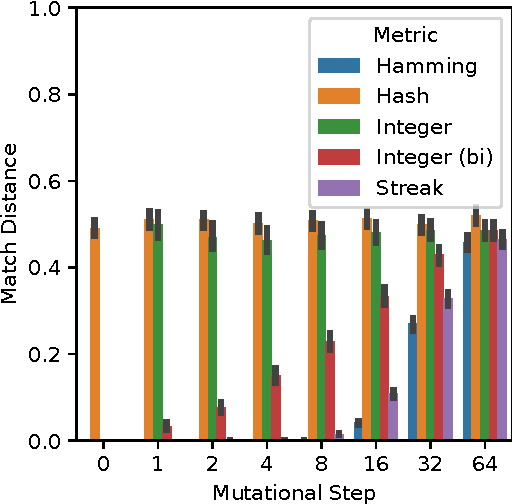
\includegraphics[width=\columnwidth]{{{mutational_walk/bitweight=0.5+seed=1+title=mutational_walk_barplot+_data_hathash_hash=8bf152d87daa9cb7+_script_fullcat_hash=982405ca713eba73+ext=}}}
\caption{
Snapshots of match distance at exponentially increasing steps from identical tags.
Error bars represent 95\% confidence intervals.
}
\label{fig:mutational_walk_barplot}

\end{center}
\end{figure}


Next, we performed mutational walks under each metric.
We began with two randomly chosen equivalent tags (mutation step zero) then applied randomly chosen one-step mutations (with the possibility of back mutation allowed) 65 times to the second tag.
We measured match distance between the two tags at each mutational step.
We performed 1000 independent mutational walks from different starting equivalent tags.

Figure \ref{fig:mutational_walk_lineplot} continuously depicts the distribution of match distances on mutational walks, with shaded areas indicating standard deviation, under different metrics.
Figure \ref{fig:mutational_walk_barplot} compares match distances at exponentially increasing steps.
Error bars indicate 95\% confidence intervals.

For the hash metric, where equivalent tags don't necessarily have low match distance, the mutational walk wanders around loose affinity.

The Spector Integer metric, where half of mutational steps wrap back around to 1.0 distance, immediately spikes up to an average match distance of 0.5.
The variance decreases with mutational steps as the distribution moves away from bias towards distances of 0 and 1.

The bidirectional integer metric experiences a greater immediate jump in variance and significantly greater mean match distance as rare mutations affecting significant bits take place (non-overlapping 95\% CI).

The
Intrestingly, contrary to as was claimed in \citep{downing2015intelligence}, the uniformified streak metric's match score under mutation actually grows significantly faster than the hamming metric's match score  (non-overlapping 95\% CI).

Because the are uniformified, the distributions all devolve to having an equivalent mean and variance.

\subsection{Target Graph Matching Evolutionary Experiment}

\begin{figure}
% \begin{minipage}{6in}
\begin{center}

\begin{minipage}{0.05\textwidth}
~
\end{minipage}%
\begin{minipage}{0.95\textwidth}
\begin{minipage}{0.05\textwidth}
~
\end{minipage}%
\begin{minipage}{0.95\textwidth}
\centering
\large
\textbf{Mean Degree}
\end{minipage}
\begin{minipage}{0.05\textwidth}
~
\end{minipage}%
\begin{minipage}{0.95\linewidth}
\begin{minipage}{0.5\textwidth}
\centering
\large
1
\end{minipage}%
\begin{minipage}{0.5\textwidth}
\centering
\large
2
\end{minipage}
\end{minipage}
\end{minipage}\\
\vspace{2ex}





\begin{minipage}{0.05\textwidth}
\large
\rotatebox[origin=c]{90}{\textbf{Structure}}
\end{minipage}%
\begin{minipage}{0.95\textwidth}
\begin{minipage}{0.05\linewidth}
\large
\rotatebox[origin=c]{90}{Irregular}
\end{minipage}%
\begin{minipage}{0.95\linewidth}
\begin{subfigure}[b]{0.5\textwidth}
\centering
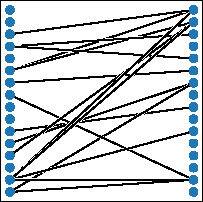
\includegraphics[width=\textwidth]{img/graph_layouts/title=irregular-1+ext=}%
\caption{
Irregular w/ mean degree 1
}
\label{fig:irregular_1}
\end{subfigure}
\begin{subfigure}[b]{0.5\textwidth}
\centering
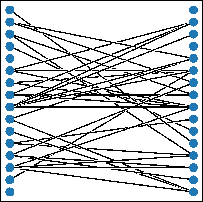
\includegraphics[width=\textwidth]{img/graph_layouts/title=irregular-2+ext=}%
\caption{
Irregular w/ mean degree 2
}
\label{fig:irregular_2}
\label{fig:irregular_degree_2}
\end{subfigure}

\end{minipage}

\vspace{2ex}

\begin{minipage}{\textwidth}

\begin{minipage}{0.05\linewidth}
\large
\rotatebox[origin=c]{90}{Regular}
\end{minipage}%
\begin{minipage}{0.95\linewidth}
\begin{subfigure}[b]{0.5\textwidth}
\centering
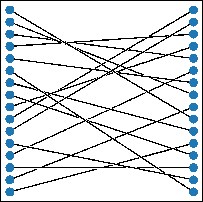
\includegraphics[width=\textwidth]{img/graph_layouts/title=regular-1+ext=}%
\caption{
Regular w/ mean degree 1
}
\label{fig:regular_degree_1}
\label{fig:regular_1}
\end{subfigure}
\begin{subfigure}[b]{0.5\textwidth}
\centering
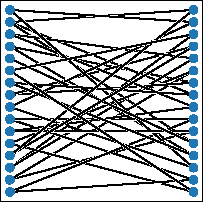
\includegraphics[width=\textwidth]{img/graph_layouts/title=regular-2+ext=}%
\caption{
Regular w/ mean degree 2
}
\label{fig:regular_degree_2}
\label{fig:regular_2}
\end{subfigure}
\end{minipage}
\end{minipage}
\end{minipage}

\caption{
Example target graph layouts used in 32-node graph-matching evolutionary experiments.
Blue dots represent tagged nodes.
Black lines represent selected-for tight affinity relationships.
Layouts differ in total number of selected-for affinities (``mean degree'') and whether selected-for affinities were evenly or randomly distributed between nodes (``structure'').
}
\label{fig:graph_layouts}


\end{center}
% \end{minipage}
\end{figure}


fitness function was based on rank matching.
Randomly generated bipartite graph as a target.
Degree, which refers to the mean number of edges attached to each node.
Regular edges were generated by randomly connecting the bipartite graph such that all left nodes and all right nodes had the same number of connections.
Irregular edges were generated by randomly adding left to right connections.
In this case, some left nodes may have more than the mean degree of edges and some left nodes may have no or fewer than the mean degree of edges.
Likewise for right nodes.
Figure \ref{fig:graph_layouts} depicts these graph layouts.

Genomes consisted of bitstring tags, sixteen representing left nodes in the bipartite graph and sixteen representing right nodes.
To evaluate the fitness of a genome, we harvested the right node tags and placed them in a tag-matching data structure that returns the ranked ordering of tag matches for a particular query tag.
Then, queried the tag-matching data structure with each left node tag in the genome.
We cut down the ranked ordering list returned to the number of the left node tag's outgoing connections in the bipartite target graph.
Fitness was calculated as the fraction of these remaining right node results that corresponded to edges in the bipartite target graph.

We performed 512-generation evolutionary runs with population size 500 and tournament size 7.
We tested combinations of two target graph types: irregular/regular edge layout and mean degree 1 or mean degree 2.
For each configuration, we surveyed each metric's performance over ten per-bit mutation rates ranging from 0.75 expected mutations per genome to 16.0 expected mutation rates per genome.
(Supplementary Figure \ref{fig:evolve_mutsweep} summarizes these results, confirming that each metric/target graph configuration shows a local maximum of performance within the range of mutation rates surveyed.)
For each metric and target graph configuration combination, we chose the most favorable mutation rate defined by sum population-maximum fitness across updates.
We ran 100 replicate evolutionary runs for each mutation rate/target graph/metric combination.

\begin{minipage}{\linewidth}
\begin{center}

\begin{minipage}{\linewidth}
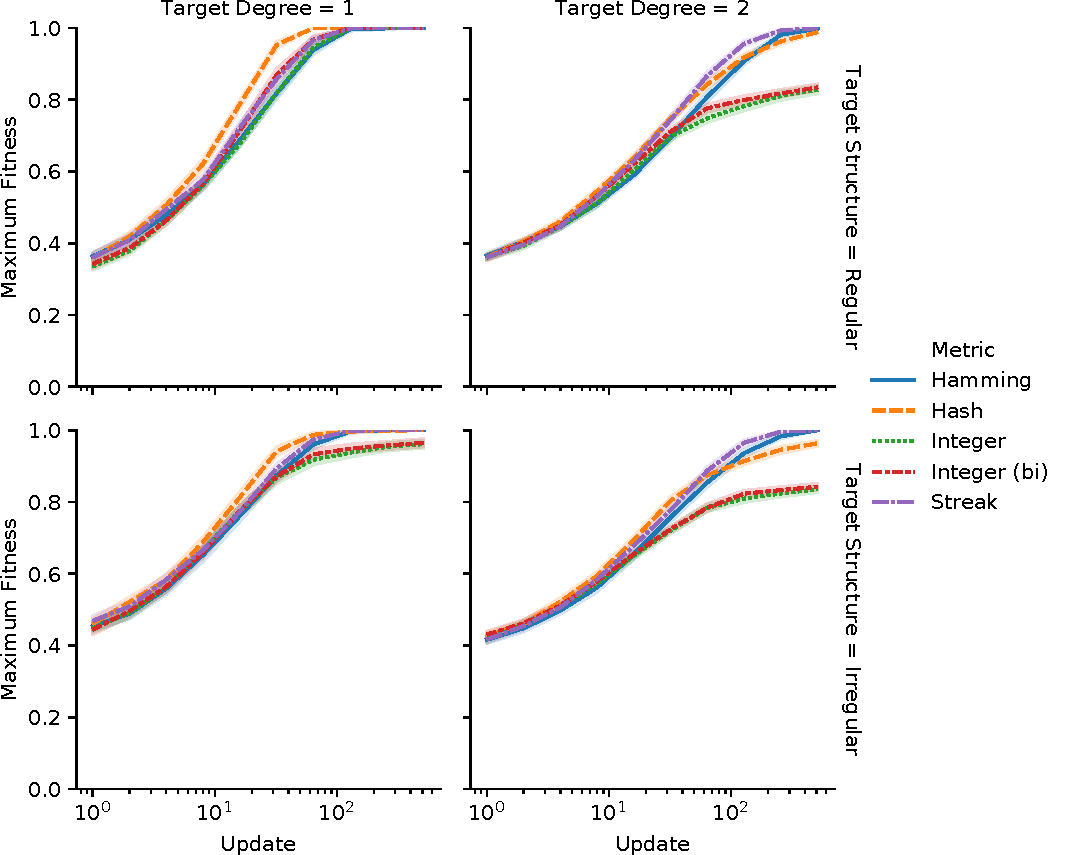
\includegraphics[width=\linewidth]{target_evolve/viz=max-fitness-line+_data_hathash_hash=673d309ab90e91d1+_script_fullcat_hash=fe3ddc711c5abfad+ext=}
\end{minipage}
\begin{minipage}{\linewidth}
\caption{
Maximum fitness by update over replicate runs for each metric's best-performing mutation rate.
Note log-scale x-axes.
Shaded area represents 95\% confidence intervals.
}
\label{fig:evolve_bests}
\end{minipage}
\end{center}
\end{minipage}


Figure \ref{fig:evolve_bests} plots population-maximum fitness across evolutionary runs.
Unsurprisingly, the hash metric performs much more poorly than all other metrics (non-overlapping 95\% confidence intervals).
The integer metrics are capable of evolving solutions to the one-to-one matching problem of the mean degree 1, regular target graph.
However, on mean degree 2 target graphs they evolve significantly poorer quality solutions.

The streak metric performs favorably or equivalently compared to all other metrics across all target graph configurations.
The streak metric yields significantly more rapid adaptive evolution than all other metrics on the regular mean degree 2 graph (non-overlapping 95\% CI).

% @AML: Once flow of paper, overall message, etc is decided, we'll most likely want to change this sub-heading
% @AML: Todo - update metric names to be consistent with rest of the paper.
\subsection{Tag-matching in a genetic programming context}

Figure/Table [X] gives the number of replicates that produced a successful SignalGP program (i.e., capable
of achieving maximum fitness) for each tag-matching metric on both the changing- and directional-signal
tasks.
For each task, we compared the number of successful replicates for each metric using pairwise Fisher's
exact tests, applying a Holm correction for multiple comparisons.
Our complete analyses, including all statistical results, can be found in our supplemental material
[cite - SGP github repository].

We observed no difference in success between the Integer and Integer-symmetric metrics on both the
changing- and directional-signal tasks.
[Statement about consistency with expectations based on previous tag-matching experiments].

On the changing-signal task, the Hamming and Streak metrics performed identically; however, on the directional-signal
task, the Streak metric performed significantly better than the Hamming metric.
[Speculation as to why].
To assess whether the Streak metric produced solutions in fewer generations than the Hamming metric,
we re-ran 200 replicates of each condition (with new random number seeds) until 50\% of the replicates
found a solution.
On the changing-signal task, we found no difference in how many generations were required for solutions
to evolve.
On the directional-signal task, however, we found that the Streak metric generally required fewer generations
than the Hamming metric to yield solutions ($p < 0.0016$).
[Statement about consistency with expectations based on previous tag-matching experiments].

Surprisingly, the Hash metric performed reasonably well on both diagnostic tasks, outperforming both
the Integer and Integer-symmetric metrics.
[Statement about consistency with expectations based on previous tag-matching experiments].
[Statement about how Hash metric is good at exploring lots of combinations very quickly, with a low
enough mutation rate].
[Of all metrics, Hash metric most susceptible to mutational meltdown at high mutation rates].

[Statement about these results overall in context of other results?].

\section{Conclusion}

Better understanding the mechanistic properties and functional implications of tag-matching criteria will help artificial life practitioners more effectively incorporate tag matching in model systems and better understand the biases imposed by those criteria.
In particular, our analyses suggests that network constraint (i.e., the degree of connectivity networks constructed by tag matching) is key to the interaction between a tag-matching scheme and problem domain.
% Better understanding tag-matching criteria willOutside of artificial life, particularly in genetic programming, where increasing the rate of adaptive evolution and evolving better-quality solutions is a key concern.

However, open questions remain with respect tag-matching criteria.
In particular, the relationships between tag-matching criteria and specificity, modularity, robustness, and the process of duplication and divergence should be explored. 
Evolvability or information-theoretical analyses may prove fruitful in this regard \citep{tarapore2015evolvability}.
How to 
%apply insight into tag-matching criteria to 
systematically design new tag-matching metrics with desirable properties also remains an open problem.

Tag-like mechanisms play a central role mediating interaction and function across the spectrum of biological scale \citep{holland2012signals}.
% Our work suggests that tag-matching systems  can have implications with respect to the structure and evolution of interaction networks.
By shining light on previously-unexplored mechanistic and evolutionary properties of tagging systems, we hope that insight into artificial tag models will translate into a more nuanced appreciation of natural systems.


\section{Acknowledgements}

Thanks to members of the DEVOLAB, in particular TODO for help with TODO.
This research was supported in part by NSF grants DEB-1655715 and DBI-0939454, and by Michigan State University through the computational resources provided by the Institute for Cyber-Enabled Research.
This material is based upon work supported by the National Science Foundation Graduate Research Fellowship under Grant No. DGE-1424871.
Any opinions, findings, and conclusions or recommendations expressed in this material are those of the author(s) and do not necessarily reflect the views of the National Science Foundation.


\footnotesize
\bibliographystyle{apalike}
\bibliography{bibl} % replace by the name of your .bib file


\end{document}
